\documentclass[letterpaper]{article}

\usepackage{hw}
\usepackage{bm}
\usepackage{amsmath}
\usepackage{graphicx}
\usepackage[colorlinks=false,urlcolor=blue]{hyperref}
\usepackage{geometry}
\geometry{margin=1in}
\usepackage{multicol}
\usepackage{paralist}
\usepackage{todonotes}
%\setlength{\marginparwidth}{2.15cm}
\usepackage{booktabs}
\usepackage{enumitem}
\usepackage{cleveref}
\usepackage{pdfpages}
\usepackage{fancyhdr}
\usepackage{fancyvrb}
\usepackage{tikz}
\usetikzlibrary{arrows}
\usepackage{graphicx}


%\DeclareMathOperator*{\argmin}{arg\,min}
%\DeclareMathOperator*{\argmax}{arg\,max}

\newcommand{\email}[1]{\href{mailto:#1@cs.cmu.edu}{#1}}

\pagestyle{fancy}
\lhead{AID :: \email{jarulraj}, \email{akalia}, \email{junwoop}}

\begin{document}

\section*{}
\begin{center}
  \centerline{\textbf{\Large Optimizing Matrix Operations Using Novel DRAM
  Access Primitives}}
  \vspace{1em}
  \textsc{\large CMU 15-745: Optimizing Compilers (Spring 2015)} \\
  \vspace{3em}
  \centerline{\large{\textbf{Group} : Joy Arulraj (\email{jarulraj}), Anuj Kalia
  (\email{akalia})}, Jun Woo Park (\email{junwoop}) }
  \vspace{1em}
\end{center}

\section{Major Changes}

There are no major changes to the goals we set out in the initial report.
We plan to implement a compiler pass to perform data structure access pattern analysis, and
then do performance evaluation to identify the impact of these DRAM access primitives.

\section{Accomplishment So Far}

The DRAM access primitives allow us to access parts of a cacheline rather than entire cachelines,
as is the case today.
This allows us to retrieve the required data (for instance, a column in a matrix) in fewer reads
compared to existing access primitives. Therefore, we end up with more efficient bandwidth
utilization and less energy consumption.

We first performed an initial evaluation of the potential performance impact of this transformation.
Specifically, we compared the time taken to compute the sum of a row and a column in a matrix laid out in
row major order. The results are shown in Figure~\ref{fig:perf}. We observe that row sum operation is several magnitudes faster compared to column sum operation. 
With the help of novel DRAM primitives, we think that the compiler can automatically identify the best
access pattern for the data structure.

\begin{figure*}
	\centering
	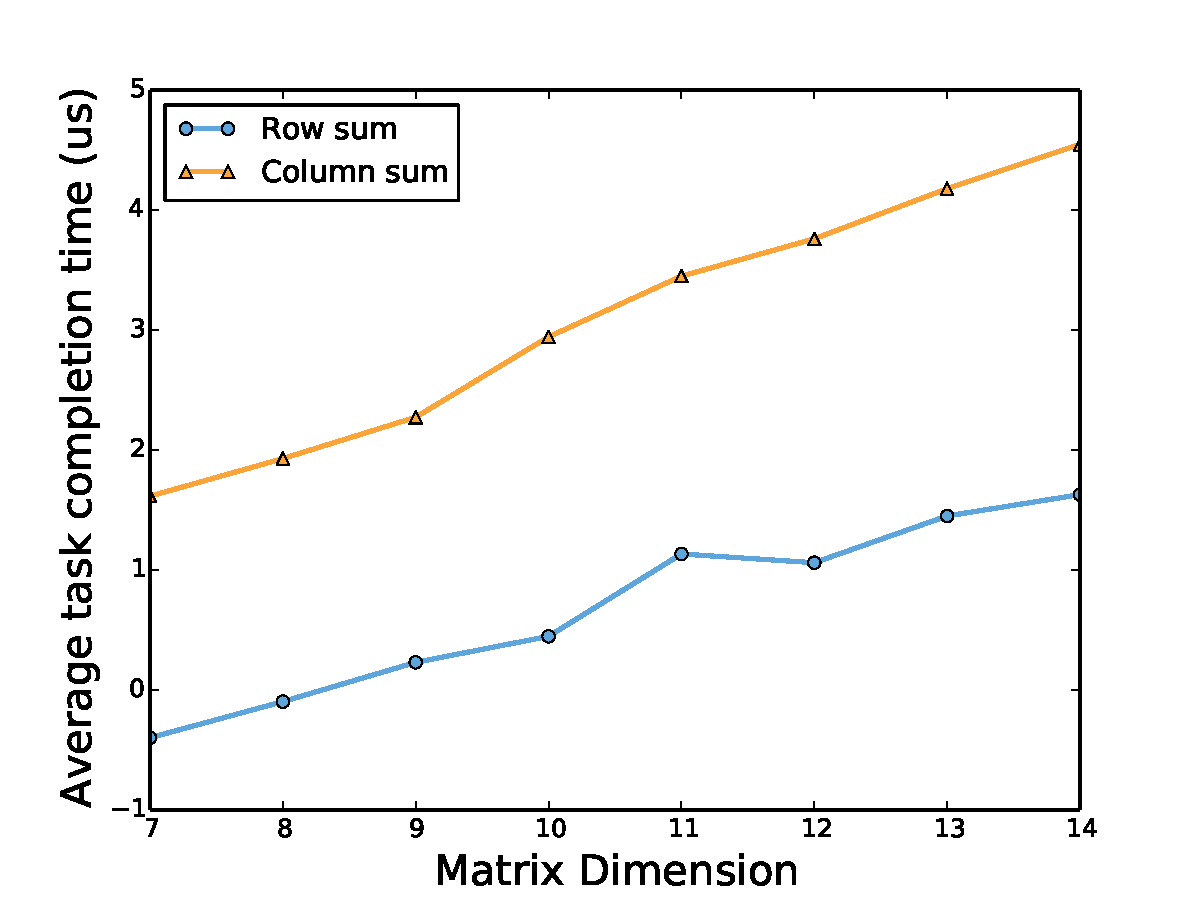
\includegraphics[scale=0.4]{rowmajor}
	\caption{Performance comparison of row and column oriented access in log scale}
	\label{fig:perf}
\end{figure*}

We have implemented an LLVM compiler pass that analyses data structure access patterns.
Currently, this targets multi-dimensional arrays of primitive data types as well as structures.
In the first stage of the pass, we parse programmer annotations to determine the data structures that
we wish to analyze. We could apply the analysis on all loads and stores, but we wanted to restrict our
analysis to important data structures that are accessed several times in loops.
Then, for each loop within a function, we analyze every load and store operation using
the Scalar Evolution (SCEV) pass to examine the scalar expressions contained in data structure
access indices. This allows us to recognize the generic induction variables in loops.
We can therefore determine the stride and offset of the access pattern. 

The output of the compiler pass on a sample program is shown below :

\begin{Verbatim}[fontsize=\small]
------------------------------
INPUT :
------------------------------
void foo(long n, long m)  {
  __attribute__((annotate(``hey, this is important''))) int A[n][m];
  struct key{
    char a;
    char b;
    char c;
  };
  __attribute__((annotate(``hey, keys''))) struct key keys[100];

  char x;
  for (long i = 0; i < n; i++) {
    for (long j = 0; j < m; j++){
      A[i][j] = 0;
      A[j][i] = 0;
      x = keys[i].a;
      keys[i].b = x;
    }
  }
}
------------------------------
OUTPUT :
------------------------------
Analysing function :: foo:
tests/a.c:i32 5           %vla = alloca i32, i32 %1, align 4    hey, this is important
tests/a.c:i32 13          %keys = alloca [100 x %struct.key], align 1   hey, keys

Inst:   store i32 0, i32* %arrayidx6, align 4
AddRec: {{0,+,(4 * %m)}<%for.cond>,+,4}<nw><%for.cond3>
ArrayRef[{0,+,1}<nuw><nsw><%for.cond>][{0,+,1}<nuw><nsw><%for.cond3>]

Inst:   store i32 0, i32* %arrayidx8, align 4
AddRec: {{0,+,4}<nuw><nsw><%for.cond>,+,(4 * %m)}<%for.cond3>
ArrayRef[{0,+,1}<nuw><nsw><%for.cond3>][{0,+,1}<nuw><nsw><%for.cond>]

Inst:   %4 = load i8* %a, align 1
AddRec: {0,+,3}<nuw><nsw><%for.cond>

Inst:   store i8 %4, i8* %b, align 1
AddRec: {1,+,3}<nw><%for.cond>
\end{Verbatim}

We are now figuring out how best to use this information to automatically transform the access patterns.

\section{Meeting Milestone}

We have implemented the compiler pass that analyses the matrix library automatically without requiring
programmer annotations about stride and offset. However, we still need to figure out how to do
a realistic performance evaluation. A first-order approximation of the performance impact is
however already seen in Figure~\ref{fig:perf}. 

\section{Surprises}

We were pleasantly surprised by the support in LLVM for analysing scalar expressions and annotations.
This helped reduce the complexity of the compiler pass.

\section{Revised Schedule}

\begin{itemize}
\item Joy Arulraj : Evaluate the performance impact of the transformations on different matrix operations.
\item Anuj Kalia : Transform the code to use the DRAM access primitives.  
\item Jun Woo Park : Examine how this transformation impacts memory level parallelism and caching behavior.
\end{itemize}

\section{Resources Needed:} 

We need some guidance on performance evaluation. We have written our own microbenchmarks and
are using the LLVM framework to implement our proposed optimizations.

%\bibliographystyle{acm}
%\bibliography{ref}

\end{document}

%%% Local Variables:
%%% mode: latex
%%% TeX-master: "."
%%% End:
